\section{Problem Statement} \label{SciRob:sec:problem}

Here we present the formal problem addressed by our method. Let the state space of the system be $\statespace$ and the action space be $\actionSpace$. The true dynamics are $\worlddynamicsdef$ produces the next state $\nextstate$ given the environment $\env$, state $\currentstate$, and action $\currentaction$. We consider the feasible discrete-time motion planning problem, which informally means finding a sequence of actions that take the system from a start configuration $\state^0$ to a goal region $\goal \subset \statespace$. In general, $\worlddynamics$ may not be known in closed-form, or it may be expensive to evaluate within a planner. Thus, we cannot solve this problem by planning with the true dynamics $\worlddynamics$.

Instead, we consider the challenge of planning with an incomplete model of the dynamics $\ourdynamics$. Since these dynamics will sometimes be inaccurate, we introduce the model-error requirement (MER) to reason about where they can be trusted. The MER is a constraint in the planning problem, to ensure that our plan only contains predictions from our dynamics $\ourdynamics$ that are $\modelerrorthreshold$-close to the true dynamics $\worlddynamics$. The model-error is defined for a given state-action $(\currentstate,\currentaction)$ using a distance function in state space $\distfname$, and is shown in Equation \eqref{Scirob:eq:modelerror}.

\begin{equation}
\modelerrordef
\label{Scirob:eq:modelerror}
\end{equation}

Using this, we define the MER itself as $\MER$. Thus, the planning problem is

\begin{equation}
  \begin{array}{ccll}
    \find & \horizon,\action^0,\dots,\lastaction & \\
    \subjectto & \nextstatepred = \ourdynamicsfunc & t \in [0,\horizon) \\
    & \modelerrorconstraint & t \in [0,\horizon) \\
    & \laststatepred \in \goal & \\
  \end{array}
  \label{Scirob:eq:planning_problem}
\end{equation}

\subsection{Classifier}

We cannot evaluate the MER directly during planning because it requires the true future state $\nextstate$.
In planning, we only know the environment, actions, and predicted states $(\env,\currentstatepred,\currentaction,\nextstatepred)$. Consequently, we need to evaluate the MER using only the information known in planning. This can be posed as the following binary classification problem:
\begin{equation}
  \begin{array}{rl}
    \classifierInputs & \env,\currentstatepred,\currentaction,\nextstatepred \\
    \classifierLabel & \MER \\
  \end{array}
  \label{Scirob:eq:strict_mer_classification_problem}
\end{equation}

Let the classifier which solves this problem be $\classifierdefNoVar$. For training this classifier, \classifierLabel can be computed using the actual $\nextstate$ recorded during data collection (Section ``\nameref{Scirob:sec:phase_two_collection}''). A diagram illustrating the inputs to the classifier and its labels is shown in Figure \ref{Scirob:fig:figure3}. Finally, given dynamics $\ourdynamics$ and classifier $\classifier$, we can approximately solve Problem \eqref{Scirob:eq:planning_problem} using motion planning (see Section ``\nameref{Scirob:sec:planning}'').

We note that the MER is conservative in the sense that we only need the final predicted $\laststatepred$ and actual state $\laststate$ to be close. Unfortunately, reasoning about only the final state in the MER would be a constraint on the entire trajectory. Such a constraint is neither tractable to learn nor amenable to planning in our scenarios. Thus, we enforce the MER for every action taken by the planner.

\begin{figure}
    \centering
    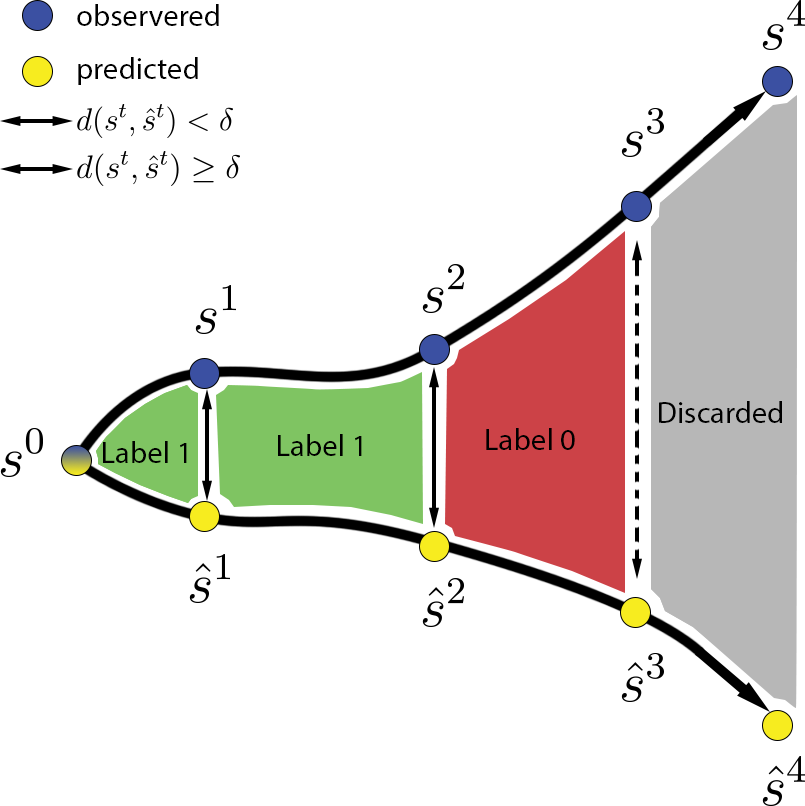
\includegraphics[width=0.5\linewidth]{Chap2/images/figure3-v2}
    \caption{Converting a trajectory into examples for training the classifier. Each large box represents a transition. In the first transition, the final states $\state^1$ and $\statepred^1$ are close, so the transition is labeled 1 (accurate). For the third transition, the initial states $\state^2$ and $\statepred^2$ are close, but the final states $\state^3$ and $\statepred^3$ are far, so this transition is labeled 0 (inaccurate). In the final transition, the initial states are far, so this transition is discarded.}
    \label{Scirob:fig:figure3}
\end{figure}

\subsection{\textit{Recovery}}

With this definition of the MER and the classifier, we also formally define what it means to be stuck, i.e. in need of recovery. This can be written as a function $\recoverydef$ which determines whether a given state, environment pair can be escaped while enforcing the MER: 
\begin{equation}
    \recoveryfuncfull
    = \begin{cases}
    0 & \exists\,\action \in \actionSpace\ \text{for which}\ \MER \\
    1 & \text{otherwise}
    \end{cases} \\
    \label{Scirob:eq:recovery}
\end{equation}

Again, we cannot compute $\recoveryfuncfull$ directly online, as it requires knowing the actual effect of executing actions. Instead, we will use an approximation to this function. Once we know if a state is in need of recovery, we can either launch the planner (if not) or perform recovery actions (if so).

\subsection{\textit{State Definition}}

In this chapter, we focus on rope manipulation tasks with $\NGrippers=1$ or $\NGrippers=2$ grippers; the state of each gripper is a point in $\reals^3$. We assume that the robot end effectors are rigidly attached to the object. The configuration of the rope is a set of $\NLinks$ points in $\reals^{3\NLinks}$. The state $s$ is then a vector of the positions of the gripper(s) and the points along the rope. The dimension of the state space is thus $\Ndim = 3 (\NGrippers + \NLinks )$.
